\chapter{Hierarchical Modeling of Non-Representative Polls}


In this chapter, I will discuss an application of hierarchical modeling
to non-representative survey sampling. As it is mentioned in the last
chapter, there is a dichotomy in modern survey research, the camp of
\emph{describers} and the camp of \emph{modelers}. However, at the heart
of modern opinion polling, for both \emph{describers} and
\emph{modelers}, is representative sampling, built around the goal that
every individual in a particular target population (e.g., registered or
likely U.S. voters) has the same probability of being sampled.
Non-representative sampling has fallen out of favor among pollsters as a
result of its inherent bias. I will show that, using an example of a
highly-biased poll on US presidential election conducted on Xbox gaming
platform, that hierarchical sampling can be used to remedy the bias and
help extract useful information from non-representative polls. This is a
joint work with David Rothschild, Sharad Goel, and Andrew Gelman, and is
published in (Wang et al. 2014).

\section{A Brief History of Representative Sampling vs
Non-representative
Sampling}\label{a-brief-history-of-representative-sampling-vs-non-representative-sampling}

The wide-scale adoption of representative polling can largely be traced
to a pivotal polling mishap in the 1936 U.S. presidential election
campaign. During that campaign, the popular magazine \emph{Literary
Digest} conducted a mail-in survey that attracted over two million
responses, a huge sample even by modern standards. The magazine,
however, incorrectly predicted a landslide victory for Republican
candidate Alf Landon over the incumbent Franklin Roosevelt. Roosevelt,
in fact, decisively won the election, carrying every state except for
Maine and Vermont. As pollsters and academics have since pointed out,
the magazine's pool of respondents was highly biased: it consisted
mostly of auto and telephone owners as well as the magazine's own
subscribers, which underrepresented Roosevelt's core constituencies
(Squire 1988). During that same campaign, pioneering pollsters,
including George Gallup, Archibald Crossley, and Elmo Roper, used
considerably smaller but representative samples to predict the election
outcome with reasonable (Gosnell 1937). Accordingly, non-representative
or ``convenience sampling'' rapidly fell out of favor with polling
experts. Methods used for sampling have evolved over time, from
address-based, in-home interview sampling in the 1930s to random digit
dialing after the growth of landlines and cellphones; nevertheless,
leading polling organizations continue to put immense effort into
obtaining representative samples.

Two recent trends spur the interest for non-representative polls. First,
representative sampling is not nearly as representative as its name
suggests, and it is becoming less so. Random digit dialing (RDD), the
standard method in modern representative polling, has suffered
increasingly high non-response rates, both due to the general public's
growing reluctance to answer phone surveys, and expanding technical
means to screen unsolicited calls (Keeter et al. 2006). By one measure,
RDD response rates have decreased from 36\% in 1997 to 9\% in 2012
(Kohut et al. 2012). With such low response rates, even if the initial
pool of targets is representative, those who ultimately answer the phone
and elect to respond are almost certainly not, calling into question the
statistical benefits of such an approach. Related to dropping response
rates is a corresponding increase in cost, in both time and money, as
one needs to contact more and more potential respondents to find one
willing to participate. The second trend driving this research is that
with recent technological innovations, it is increasingly convenient and
cost-effective to collect large numbers of highly non-representative
samples via online surveys. What took several months for the
\emph{Literary Digest} editors to collect in 1936 can now take only a
few days and can cost just pennies per response. The challenge, of
course, is to extract meaningful signal from these unconventional
samples.

It is worth noting that the so-called ``Big Data'' is more often than
not a convenient sample, with potentially huge selection bias. Without
adequately addressing this issue first, any conclusion drawn from big
data analysis might be misleading.

\subsection{Xbox Data}\label{xbox-data}

The analysis is based on an opt-in poll continuously available on the
Xbox gaming platform during the 45 days preceding the 2012 U.S.
presidential election. Each day, three to five questions were posted,
one of which gauged voter intention with the standard query, ``If the
election were held today, who would you vote for?''. Respondents were
allowed to answer at most once per day. The first time they participated
in an Xbox poll, respondents were additionally asked to provide basic
demographic information about themselves, including their sex, race,
age, education, state, party ID, political ideology, and for whom they
voted in the 2008 presidential election. In total, 750,148 interviews
were conducted with 345,858 unique respondents---over 30,000 of whom
completed five or more polls---making this one of the largest ever
election panel studies.

\begin{figure}[p!]
  \centering
  \includegraphics[width=\textwidth]{"xbox_electorate_demo_comp"}
  \caption{A comparison of the demographic, partisan, and 2008 vote
    distribution in the Xbox dataset and the 2012 electorate (as
    measured by adjusted exit polls). The sex and age distributions, as one might expect, exhibit
  considerable differences.}
  \label{fig:demo_comp}
\end{figure}

\begin{figure}[p!]
  \centering
  \includegraphics[width=.8\textwidth]{"raw_response"}
  \caption{Daily (unadjusted) Xbox estimates of two-party Obama support during
    the 45 days leading up to the 2012 presidential election, which suggest a
    landslide victory for Mitt Romney. The dotted blue line indicates a
    consensus average of traditional polls (the daily aggregated polling results from Pollster.com), the horizontal dashed line at 52\%
    indicates the actual two-party vote share obtained by Barack Obama, and the
    vertical dotted lines give the dates of the three presidential debates.}
  \label{fig:raw_responses}
\end{figure}

Despite the large sample size, the pool of Xbox respondents is far from
representative of the voting population.
Figure\textasciitilde{}\ref{fig:demo_comp} compares the demographic
composition of the Xbox participants to that of the general electorate,
as estimated via the 2012 national exit poll. For ease of
interpretation, in Figure\textasciitilde{}\ref{fig:demo_comp} states are
grouped into 4 categories: (1) battleground states (Colorado, Florida,
Iowa, New Hampshire, Ohio, and Virginia), the five states with the
highest amounts of TV spending plus New Hampshire, which had the highest
per-capita spending; (2) quasi-battleground states (Michigan, Minnesota,
North Carolina, Nevada, New Mexico, Pennsylvania, and Wisconsin), which
round out the states where the campaigns and their affiliates made major
TV buys; (3) solid Obama states (California, Connecticut, District of
Columbia, Delaware, Hawaii, Illinois, Maine, Maryland, Massachusetts,
New Jersey, New York, Oregon, Rhode Island, Vermont, and Washington);
and (4) solid Romney states (Alabama, Alaska, Arizona, Arkansas,
Georgia, Idaho, Indiana, Kansas, Kentucky, Louisiana, Mississippi,
Missouri, Montana, Nebraska, North Dakota, Oklahoma, South Carolina,
South Dakota, Tennessee, Texas, Utah, West Virginia, and Wyoming). The
most striking differences are for age and sex. As one might expect,
young men dominate the Xbox population: 18-to-29-year-olds comprise 65\%
of the Xbox dataset, compared to 19\% in the exit poll; and men make up
93\% of the Xbox sample but only 47\% of the electorate. Political
scientists have long observed that both age and sex are strongly
correlated with voting preferences (Kaufmann and Petrocik 1999), and
indeed these discrepancies are apparent in the unadjusted time-series of
Xbox voter intent shown in Figure \ref{fig:raw_responses}. In contrast
to estimates based on traditional, representative polls (indicated by
the dotted blue line in Figure \ref{fig:raw_responses}), the uncorrected
Xbox sample suggests a landslide victory for Mitt Romney, reminiscent of
the infamous \emph{Literary Digest} error.

\section{Estimating voter intent with multilevel regression and
poststratification}\label{estimating-voter-intent-with-multilevel-regression-and-poststratification}

\subsection{Multilevel regression and
poststratification}\label{multilevel-regression-and-poststratification}

To transform the raw Xbox data into accurate estimates of voter intent
in the general electorate, I make use of the rich demographic
information that respondents provide. In particular I
\emph{poststratify} the raw Xbox responses to mimic a representative
sample of likely voters. Poststratification is a popular method for
correcting for known differences between sample and target populations
(Little 1993). The core idea is to partition the population into cells
(e.g., based on combinations of various demographic attributes), use the
sample to estimate the response variable within each cell, and finally
to aggregate the cell-level estimates up to a population-level estimate
by weighting each cell by its relative proportion in the population.
Using \(y\) to indicate the outcome of interest, the poststratification
estimate is defined by,

\begin{equation*}
\hat{y}^{\text{PS}}=\frac{\sum_{j=1}^JN_j\hat{y}_j}{\sum_{j=1}^JN_j}
\end{equation*}

\noindent where \(\hat{y}_j\) is the estimate of \(y\) in cell \(j\),
and \(N_j\) is the size of the \(j\)-th cell in the population. An
estimate of \(y\) can be analogously derived at any subpopulation level
\(s\) (e.g., voter intent in a particular state) by

\begin{equation*}
\hat{y}_s^{\text{PS}}=\frac{\sum_{j\in J_s}N_j\hat{y}_j}{\sum_{j\in J_s}N_j}
\end{equation*}

\noindent where \(J_s\) is the set of all cells that comprise \(s\). As
is readily apparent from the form of the poststratification estimator,
the key is to obtain accurate cell-level estimates, as well as estimates
for the cell sizes.

One of the most common ways to generate cell-level estimates is to
simply average sample responses within each cell. If it is assumed that
within a cell the sample is drawn at random from the larger population,
this yields an unbiased estimate. However, this assumption of cell-level
simple random sampling is only reasonable when the partition is
sufficiently fine; on the other hand, as the partition becomes finer,
the cells become sparse, and the empirical sample averages become
unstable. I address these issues by instead generating cell-level
estimates via a regularized regression model, namely multilevel
regression.

This combined model-based poststratification strategy, known as
multilevel regression and poststratification (MRP), has been used to
obtain accurate small-area subgroup estimates, such as for public
opinion and voter turnout in individual states and demographic subgroups
{[}Park, Gelman, and Bafumi (2004);Lax and Phillips (2009);Ghitza and
Gelman (2013)\}.

More formally, applying MRP in this setting comprises two steps. First a
Bayesian hierarchical model is fit to obtain estimates for sparse
poststratification cells; second, one averages over the cells, weighting
by a measure of forecasted voter turnout, to get state and
national-level estimates. Specifically, I generate the cells by
considering all possible combinations of sex (2 categories), race (4
categories), age (4 categories), education (4 categories), state (51
categories), party ID (3 categories), ideology (3 categories) and 2008
vote (3 categories), which partition the data into 176,256 cells. \{All
demographic variables are collected prior to respondents' first poll,
alleviating concerns that respondents may adjust their demographic
responses to be inline with their voter intention (e.g., a new Obama
supporter switching his or her party ID from Republican to Democrat). I
fit two, nested multilevel logistic regressions to estimate candidate
support in each cell. The first of the two models predicts whether a
respondent supports a major-party candidate (i.e., Obama or Romney), and
the second predicts support for Obama given that the respondent supports
a major-party candidate. Following the notation of (Gelman and Hill
2007), the first model is given by

\begin{align}\label{eqn:m1}
  \text{Pr}(Y_i \in \, &\{\text{Obama, Romney}\})=\nonumber\\
  &\text{logit}^{-1}\big(\alpha_0+  \alpha_1\text{(state last vote share)} \\
  &+ a^{\text{state}}_{j[i]}+a^{\text{edu}}_{j[i]}+a^{\text{sex}}_{j[i]}+a^{\text{age}}_{j[i]}
  +a^{\text{race}}_{j[i]}+a^{\text{party ID}}_{j[i]}
  +b^{\text{ideology}}_{j[i]} + b^{\text{last vote}}_{j[i]} \big)\nonumber
\end{align}

where \(\alpha_0\) is the fixed baseline intercept, and \(\alpha_1\) is
the fixed slope for Obama's fraction of two-party vote share in the
respondent's state in the last presidential election. The terms
\(a^{\text{state}}_{j[i]}\), \(a^{\text{edu}}_{j[i]}\),
\(a^{\text{sex}}_{j[i]}\) and so on---which in general is denote by
\(a^{\text{var}}_{j[i]}\)---correspond to varying coefficients
associated with each categorical variable. Here the subscript \(j[i]\)
indicates the cell to which the \(i\)-th respondent belongs. For
example, \(a^{\text{age}}_{j[i]}\) takes values from
\(\{a^{\text{age}}_{18-29}, a^{\text{age}}_{30-44}, a^{\text{age}}_{45-64}, a^{\text{age}}_{65+}\}\)
depending on the cell membership of the \(i\)-th respondent. The varying
coefficients \(a_{j[i]}^{\text{var}}\) are given independent prior
distributions

\begin{equation*}
a^{\text{var}}_{j[i]}\sim N(0,\sigma^2_\text{var}).
\end{equation*}

\noindent To complete the full Bayesian specification, the variance
parameters are assigned a hyperprior distribution

\begin{equation*}\sigma^2_\text{var}\sim \text{inv-}\chi^2(\nu, \sigma_0^2),
\end{equation*}

\noindent with a weak prior specification for the remaining parameters,
\(\nu\) and \(\sigma_0\). The benefit of using a multilevel model is
that estimates for relatively sparse cells can be improved through
``borrowing strength'' from demographically similar cells that have
richer data. Similarly, the second model is defined by

\begin{align}  \label{eqn:m2}
  \text{Pr}(Y_i = \, &\text{Obama} \, |\, Y_i\in\{\text{Obama, Romney}\})=\nonumber\\
  &\text{logit}^{-1}\big(\beta_0+ \beta_1\text{(state last vote share)} \\
  & + b^{\text{state}}_{j[i]}+b^{\text{edu}}_{j[i]}+b^{\text{sex}}_{j[i]}+b^{\text{age}}_{j[i]}
  +b^{\text{race}}_{j[i]}+b^{\text{party ID}}_{j[i]} +
  b^{\text{ideology}}_{j[i]} + b^{\text{last vote}}_{j[i]}
 \big)\nonumber
\end{align}

\noindent and

\begin{align*}
  b^{\text{var}}_{j[i]}&\sim N(0,\eta^2_\text{var}),\\
  \eta^2_\text{var}&\sim \text{inv-}\chi^2(\mu, \eta_0^2).
  \end{align*}

Jointly, Eqs.\textasciitilde{}\eqref{eqn:m1} and \eqref{eqn:m2} define a
Bayesian model that describes the data. Ideally, a fully Bayesian
analysis would be performed to obtain the posterior distribution of the
parameters. However, for computational convenience, I use the
approximate marginal maximum likelihood estimates obtained from the
\texttt{glmer()} function in the \texttt{R} package \texttt{lme4}
(Bates, Maechler, and Bolker 2013).

Having detailed the multilevel regression step, I now turn to
poststratification, where cell-level estimates are weighted by the
proportion of the electorate in each cell and aggregated to the
appropriate level (e.g., state or national). To compute cell weights,
cross-tabulated population data is needed. One commonly used source for
such data is the Current Population Survey (CPS); however, the CPS does
not includes some key poststratification variables, such as party
identification. I thus instead use exit poll data from the 2008
presidential election. Exit polls are conducted on election day outside
voting stations to record the choices of exiting voters, and they are
generally used by researchers and news media to analyze the demographic
breakdown of the vote (after a post-election adjustment that aligns the
weighted responses to the reported state-by-state election results). In
total, 101,638 respondents were surveyed in the state and national exit
polls. I use the exit poll from 2008, not 2012, because this means that
in theory the method as described here could have been used to generate
real-time predictions during the 2012 election campaign. Admittedly,
this approach puts my prediction at a disadvantage since the demographic
shifts of the intervening four years cannot be captured. While combining
exit poll and CPS data would arguably yield improved results, for
simplicity and transparency I exclusively use the 2008 exit poll
summaries for poststratification.

\subsection{National and State Voter
Intent}\label{national-and-state-voter-intent}

Figure\textasciitilde{}\ref{fig:national_snap} shows the adjusted
two-party Obama support for the last 45 days of the election. \%The
daily voter intents for two-party Obama support at the national level
are \%illustrated in Figure \ref{fig:national_snap}. Compared with the
uncorrected estimates in Figure \ref{fig:raw_responses}, the
MRP-adjusted estimates yield a much more reasonable timeline of Obama's
standing over the course of the final weeks of the campaign. With a
clear advantage at the beginning, Obama's support slipped rapidly after
the first presidential debate---though never falling below 50\%---and
gradually recovered, building up a decisive lead in the final days.

On the day before the election, the estimate of voter intent is off by a
mere 0.6 percentage points from the actual outcome (indicated by the
dotted horizontal line). Voter intent in the weeks prior to the election
does not directly equate to an estimate of vote share on election
day---a point I return to in Section\textasciitilde{}\ref{sec:forecast}.
As such, it is difficult to evaluate the accuracy of the full
time-series of estimates. Nonetheless, note that the estimates are not
only intuitively reasonable, but that they are also inline with
prevailing estimates based on traditional, representative polls. In
particular, the estimates roughly track---and are even arguably better
than---those from Pollster.com, one of the leading poll aggregators
during the 2012 campaign.

\begin{figure}[p!]
  \centering
  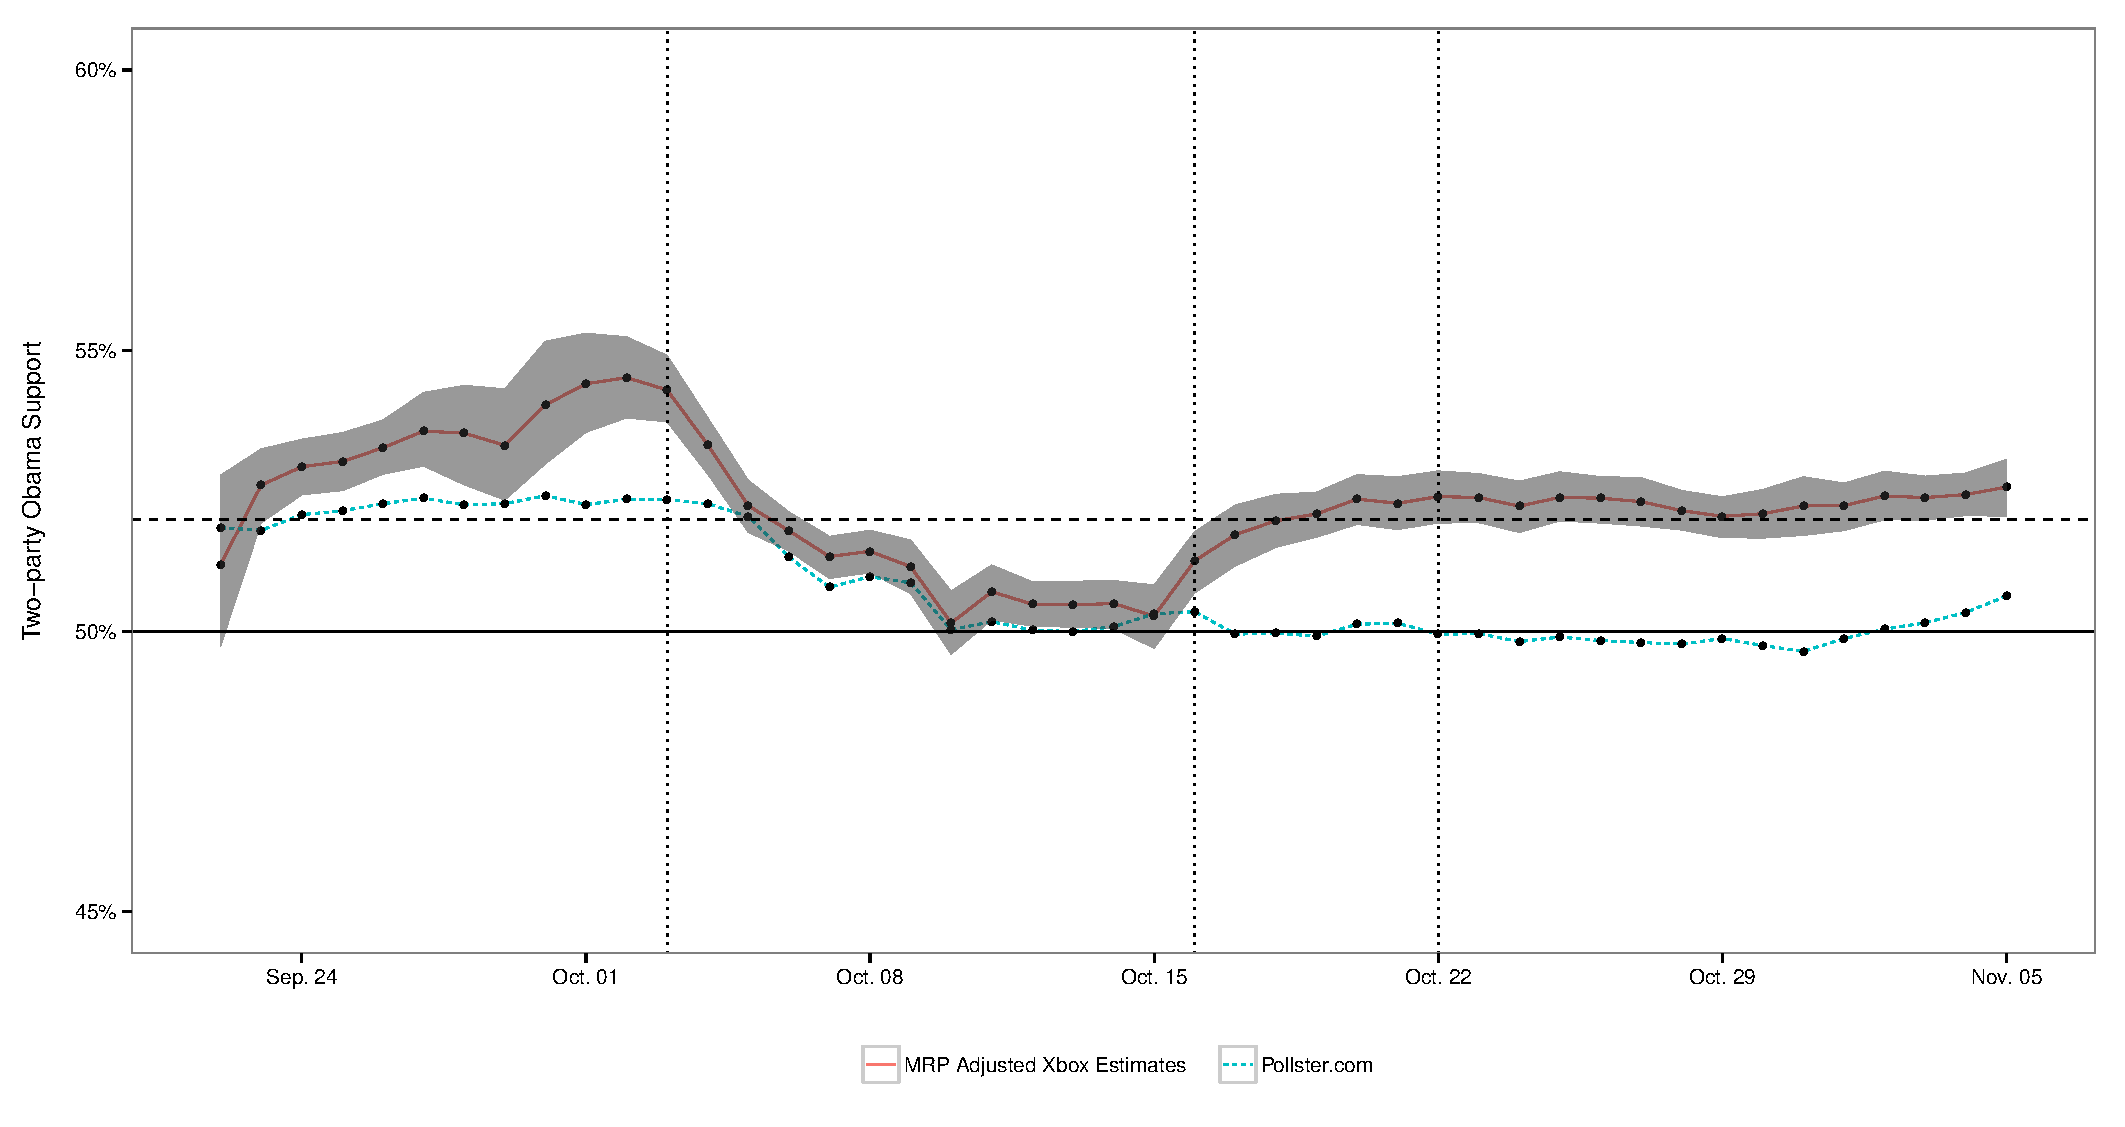
\includegraphics[width=.8\textwidth]{mrp_snapshots_national}
  \caption{National MRP-adjusted voter intent of two-party Obama support over
    the 45-day period and the associated 95\% confidence bands. The horizontal
    dashed line indicates the actual two-party Obama vote share. The three
    vertical dotted lines indicate the presidential debates. Compared with the raw
    responses in Figure \ref{fig:raw_responses}, the MRP-adjusted voter intent
    is much more reasonable, and voter intent in the last few days is very
    close to the actual outcome. For comparison, the daily aggregated polling
    results from Pollster.com, shown as the blue dotted line, are further away from the actual vote share
    than the estimates generated from the Xbox data in the last few days.}
  \label{fig:national_snap}
\end{figure}

National vote share receives considerable media attention, but
state-level estimates are particularly relevant for many stakeholders
given the role of the Electoral College in selecting the winner
(Rothschild 2013). forecast the joint probability of victory for each
candidate in Forecasting state-by-state races is a challenging problem
due to the interdependencies in state outcomes, \%and the joint
electoral votes has not yet become the standard forecast the logistical
difficulties of measuring state-level vote preference, and the effort
required to combine information from various sources (Lock and Gelman
2010). The MRP framework, however, provides a straightforward
methodology for generating state-level results. Namely, I use the same
cell-level estimates employed in the national estimate, as generated via
the multilevel model in Eqs.~\eqref{eqn:m1} and \eqref{eqn:m2}, and I
then poststratify to each state's demographic composition. In this
manner, the Xbox responses can be used to construct estimates of voter
intent over the last 45 days of the campaign for all 51 Electoral
College races.

Figure \ref{fig:state_snap} shows two-party Obama support for the 12
states with the most electoral votes. The state timelines share similar
trends (e.g., support for Obama dropping after the first debate), but
also have their own idiosyncratic movements, an indication of a
reasonable blend of national and state-level signals. To demonstrate the
accuracy of the MRP-adjusted estimates, I plot, in dotted blue lines in
Figure\textasciitilde{}\ref{fig:state_snap}, the estimates generated by
Pollster.com, which are broadly consistent with the state-level MRP
estimates. Moreover, across the 51 Electoral College races, the mean and
median absolute errors of the estimates on the day before the election
are just 2.5 and 1.8 percentage points, respectively.

\begin{figure}[p!]
  \centering
  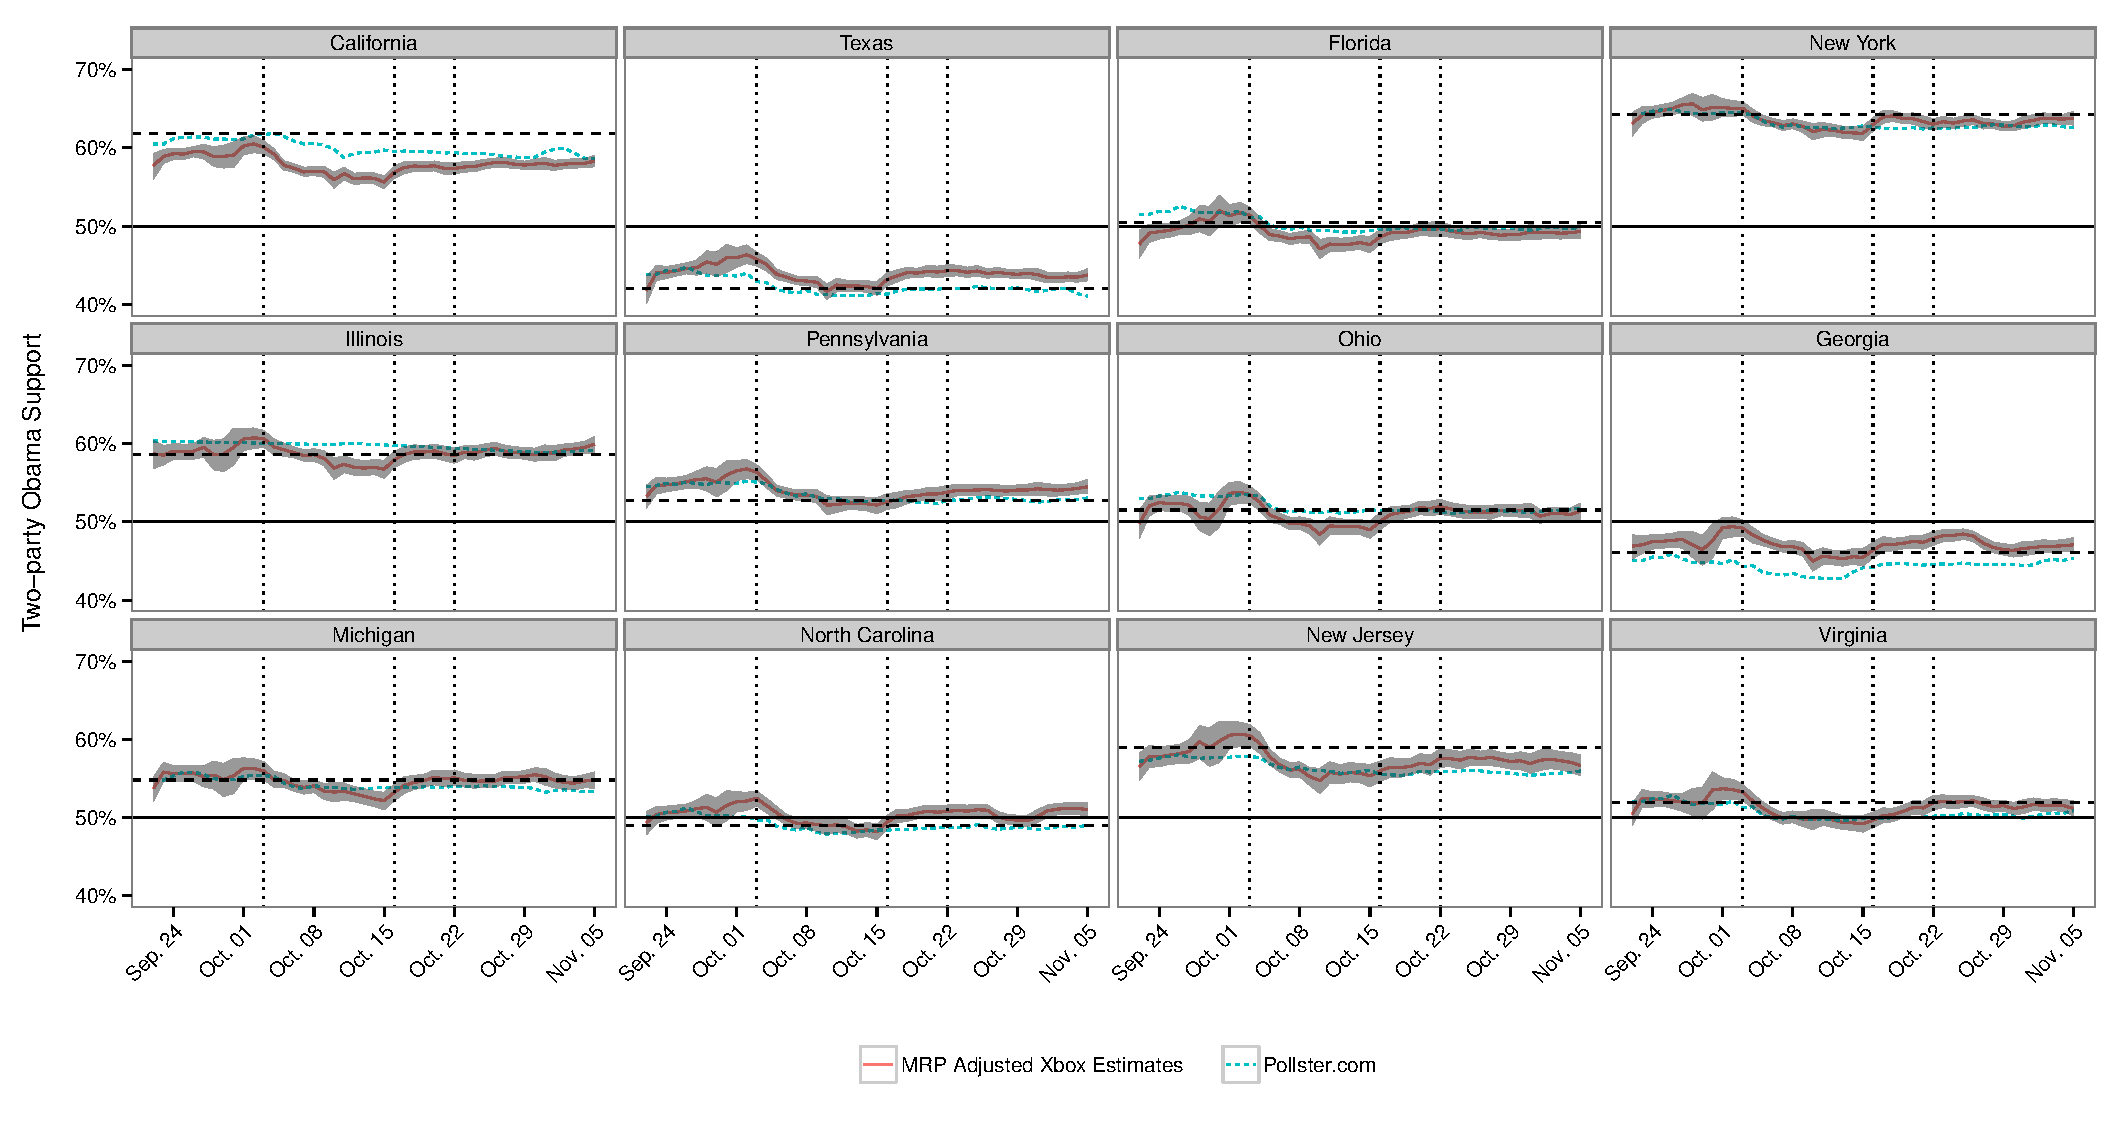
\includegraphics[width=15cm]{mrp_snapshots_state}
  \caption{MRP-adjusted daily voter intent for the 12 states with the most electoral
    votes, and the associated 95\% confidence bands. The horizontal dashed lines
    in each panel give the actual two-party Obama vote shares in that
    state. The mean and median absolute errors of the last day voter intent
    across the 51 Electoral College races are 2.5 and 1.8 percentage points,
    respectively. The state-by-state daily aggregated polling results from
    Pollster.com, given in the dotted blue lines, are broadly consistent with
    the estimates from the Xbox data.}
  \label{fig:state_snap}
\end{figure}

\subsection{Voter intent for demographic
subgroups}\label{voter-intent-for-demographic-subgroups}

Apart from Electoral College races, election forecasting often focuses
on candidate preference among demographic subpopulations. Such forecasts
are of significant importance in modern political campaigns, which often
employ targeted campaign strategies (Hillygus and Shields 2009). In the
highly non-representative Xbox survey, certain subpopulations are
heavily underrepresented and plausibly suffer from strong self-selection
problems. This begs the question, how accurate the estimates for older
women based on a platform that caters to mostly young men?

\begin{figure} \centering
  \includegraphics[width=\textwidth]{"demo_group_marginals"} \caption{Comparison
  of two-party Obama vote share for various demographic subgroups, as estimated
  from the 2012 national exit poll and from the Xbox data on the day before the
  election.  } \label{fig:marginal_comp} \end{figure}

\begin{figure}
  \centering
  \includegraphics[width=.6\textwidth]{"demo_groups_two_way_interaction"}
  \caption{Two-party Obama support as estimated from
  the 2012 national exit poll and from the Xbox data on the day before the election,
    for various two-way interaction demographic subgroups (e.g., 65+ year-old women).
    The sizes of the dots are proportional to the
    population sizes of the corresponding subgroups. Subgroups within the same
    two-way interaction category (e.g., age by sex) have the same color.}
  \label{fig:two_way_comp}
\end{figure}

It is straightforward in MRP to estimate voter intent among any
collection of demographic cells: I again use the same cell-level
estimates as in the national and state settings, but poststratify to the
desired target population. For example, to estimate voter intent among
women, the poststratification weights are based on the relative number
of women in each demographic cell. To illustrate this approach, I
compute Xbox estimates of Obama support for each level of the
categorical variables (e.g., males, females, Whites, Blacks, etc.) on
the day before the election, and compare those with the actual voting
behavior of those same groups as estimated by the 2012 national exit
poll. As seen in Figure\textasciitilde{}\ref{fig:marginal_comp}, the
Xbox estimates are remarkably accurate, with a median absolute
difference of 1.5 percentage points between the Xbox and the exit poll
numbers. Note that Respondents' 2008 vote was not asked on the 2012 exit
poll, so I exclude that comparison from
Figure\textasciitilde{}\ref{fig:marginal_comp}.

Not only do the Xbox data facilitate accurate estimation of voter intent
across these single-dimensional demographic categories, but they also do
surprisingly well at estimating two-way interactions (e.g., candidate
support among 18--29 year-old Hispanics, and liberal college graduates).
Figure\textasciitilde{}\ref{fig:two_way_comp} shows this result,
plotting the Xbox estimates against those derived from the exit polling
data for each of the 149 two-dimensional demographic subgroups. Note
that state contestedness is excluded from the two-way interaction groups
since the 2012 state exit polls are not yet available, and the 2012
national exit poll does not have enough data to reliably estimate state
interactions; 2008 vote is also excluded, as it was not asked in the
2012 exit poll. The ``other'' race category was also dropped as it was
not consistently defined across the Xbox and exit poll datasets. Most
points lie close to the diagonal, indicating that the Xbox and exit poll
estimates are in agreement. Specifically, for women who are 65 and
older---a group whose preferences one might a priori believe are hard to
estimate from the Xbox data---the difference between Xbox and the exit
poll is a mere one percentage point (49.5\% and 48.5\%, respectively).
Across all the two-way interaction groups, the median absolute
difference is just 2.4 percentage points. As indicated by the size of
the points in Figure\textasciitilde{}\ref{fig:two_way_comp}, the largest
differences occur for relatively small demographic subgroups (e.g.,
liberal Republicans), for which both the Xbox and exit poll estimates
are less reliable. For the 30 largest demographic subgroups,
Figure\textasciitilde{}\ref{fig:30groups} lists the differences between
Xbox and exit poll estimates. Among these largest subgroups, the median
absolute difference drops to just 1.9 percentage points.

\begin{figure}
  \centering
  \includegraphics{"two_way_interaction_diff"}
  \caption{Differences between the Xbox MRP-adjusted estimates and
    the exit poll estimates for the 30 largest two-dimensional demographic
    subgroups, ordered by the difference.  Positive values indicate the Xbox
    estimate is larger than the corresponding exit poll estimate.  Among these 30
    subgroups, the median and mean absolute differences are 1.9 and 2.2
    percentage points, respectively.}
  \label{fig:30groups}
\end{figure}

\section{Forecasting Election Day
Outcome}\label{forecasting-election-day-outcome}

\subsection{Converting Voter Intent to
Forecasts}\label{converting-voter-intent-to-forecasts}

As mentioned above, daily estimates of voter intent do not directly
correspond to estimates of vote share on election day. There are two key
factors for this deviation. First, opinion polls (both representative
and non-representative ones) only gauge voter preference on the
particular day when the poll is conducted, with the question typically
phrased as, ``if the election were held today.'' Political scientists
and pollsters have long observed that such stated preferences are prone
to several biases, including the anti-incumbency bias, in which the
incumbent's polling numbers tend to be lower than the ultimate outcome
(Campbell 2008), and the fading early lead bias, in which a big lead
early in the campaign tends to diminish as the election gets closer
(Erikson and Wlezien 2008). Moreover, voters' attitudes are affected by
information revealed over the course of the campaign, so preferences
weeks or months before election day are at best a noisy indicator of
one's eventual vote. Second, estimates of vote share require a model of
likely voters. That is, opinion polls measure preferences among a
hypothetical voter pool, and are thus accurate only to the extent that
this pool captures those who actually turn out to vote on election day.
Both of these factors introduce significant complications in forecasting
election day outcomes.

To convert daily estimates of voter intent to election day
predictions---which I hereafter refer to as ({\textbf{???}}) voter
intent---I compare daily voter intent in previous elections to the
ultimate outcomes in those elections. Specifically, I collected
historical data from three previous U.S. presidential elections, in
2000, 2004, and 2008. For each year, I obtained top-line (i.e., not
individual-level) national and state estimates of voter intent from all
available polls conducted in those elections. The polling data are
obtatined from \url{Pollster.com} and \url{RealClearPolitics.com}. From
this collection of polling data, I then constructed daily estimates of
voter intent by taking a moving average of the poll numbers, in a
similar manner to the major poll aggregators. Note that I rely on
traditional, representative polls to reconstruct historical voter
intent; in principle, however, I could have started with
non-representative polls if such data were available in previous
election cycles.

I next infer a mapping from voter intent to election outcomes by
regressing election day vote share on the historical time-series of
voter intent. The key difference between the approach in this chapter
and previous related work (Erikson and Wlezien 2008; Rothschild 2009) is
that I explicitly model state-level correlations, via nested national
and state models and correlated error terms. Specifically, I first fit a
national model given by

\begin{align*}
  y^{\text{US}}_{e}=a_0+a_1 x^{\text{US}}_{t,e}+
  a_2|x^{\text{US}}_{t,e}|x^{\text{US}}_{t,e} +
  a_3tx^{\text{US}}_{t,e} + \eta(t,e)
  \end{align*}

\noindent where \(y^{\text{US}}_{e}\) is the national election day vote
share of the incumbent party candidate in election year \(e\),
\(x^{\text{US}}_{t,e}\) is the national voter intent of the incumbent
party candidate at \(t\) days before the election in year \(e\), and
\(\eta \sim N(0,\sigma^2)\) is the error term. Both
\(y^{\text{US}}_{e}\) and \(x^{\text{US}}_{t,e}\) are offset by 0.5, so
the values run from \$-\$0.5 to 0.5 rather than 0 to 1. The term
involving the absolute value of voter intent pulls the vote share
prediction toward 50\%, capturing the diminishing early lead effect. I
do not include a main effect for time since it seems unlikely that the
number of days until the election itself contributes to the final vote
share directly, but rather time contributes through its interaction with
the voter intent (which it is include in the model).

Similarly, the state model is given by

\begin{align*}
  y_{s,e}^{\text{ST}}=b_0+b_1 x_{s,t,e}^{\text{ST}}+
  b_2|x_{s,t,e}^{\text{ST}}|x_{s,t,e}^{\text{ST}} +
  b_3tx_{s,t,e}^{\text{ST}} + \varepsilon(s,t,e)
\end{align*}

where \(y_{s,e}^{\text{ST}}\) is the election day state vote share of
the state's incumbent party candidate at day \(t\),
\(x_{s,t,e}^{\text{ST}}\) is the state voter intent at day \(t\), and
\(\epsilon\) is the error term. The outcome \(y_{s,e}^{\text{ST}}\) is
offset by the national projected vote share on that day as fit with the
national calibration model, and \(x_{s,t,e}^{\text{ST}}\) is offset by
that day's national voter intent. Furthermore, I impose two restrictions
on the magnitude and correlation structure of the error term
\(\varepsilon(s,t,e)\). First, since the uncertainty naturally decreases
as the election gets closer (as \(t\) becomes smaller), I apply the
heteroscedastic structure \(\text{Var}(\varepsilon(s,t,e))=(t+a)^2\),
where \(a\) is a constant to be estimated from the data. Second, the
state-specific movements within each election year are allowed to be
correlated. For simplicity, and as in (Chen, Ingersoll, and Kaplan
2008), I assume these correlations are uniform (i.e., all pairwise
correlations are the same), which creates one more parameter to be
estimated from the data. I fit the full calibration model with the
\texttt{gls()} function in the \texttt{R} package \texttt{nlme}
(Pinheiro et al. 2012).

In summary, the procedure for generating election day forecasts proceeds
in three steps:

\begin{enumerate}
\item Estimate the joint distribution of state and national voter intent by applying MRP to the Xbox data,
as described in Section~\ref{sec:mrp}.
\item Fit the nested calibration model described above on historical data to obtain point estimates for the parameters, including
estimates for the error terms.
\item Convert the distribution of voter intent to election day forecasts via the fitted calibration model.
\end{enumerate}

\subsection{National and state election day
forecasts}\label{national-and-state-election-day-forecasts}

Figure \ref{fig:proj_state} plots the projected vote shares and
pointwise 95\% confidence bands over time for the 12 states with the
most electoral votes. Though these time-series look quite reasonable, it
is difficult to assess their accuracy as there are no ground truth
estimates to compare with in the weeks prior to the election. As a
starting point, I compare the state-level estimates to those generated
by prediction markets, which are widely considered to be among the most
accurate sources for political predictions\textasciitilde{}(Rothschild
2013; Wolfers and Zitzewitz 2004). For each state, prediction markets
produce daily probabilities of victory. Though
Figure\textasciitilde{}\ref{fig:proj_state} plots the forecasts in terms
of expected vote share, this estimation procedure in fact yields the
full distribution of outcomes, and so I can likewise convert my
estimates to probabilistic forecasts.
Figure\textasciitilde{}\ref{fig:pm_comp} shows this comparison, where
the prediction market estimate is derived by averaging the two largest
election markets, Betfair and Intrade. My probabilistic estimates are
largely consistent with the prediction market probabilities. In fact,
for races with little uncertainty (e.g., Texas and Massachusetts), the
Xbox estimates do not seem to suffer from the long-shot bias common to
prediction markets (Rothschild 2009), and instead yield probabilities
closer to 0 or 1. For tighter races, the Xbox estimates---although still
highly correlated with the prediction market probabilities---look more
volatile, especially in the early part of the 45-day period. Since the
ground truth is not clearly defined, it is difficult to evaluate which
method---Xbox or prediction markets---yields better results. From a
Bayesian perspective, if one believes the stability shown by prediction
markets, this could be incorporated into the structure of the Xbox
calibration model.

\begin{figure}[p!]
  \centering
  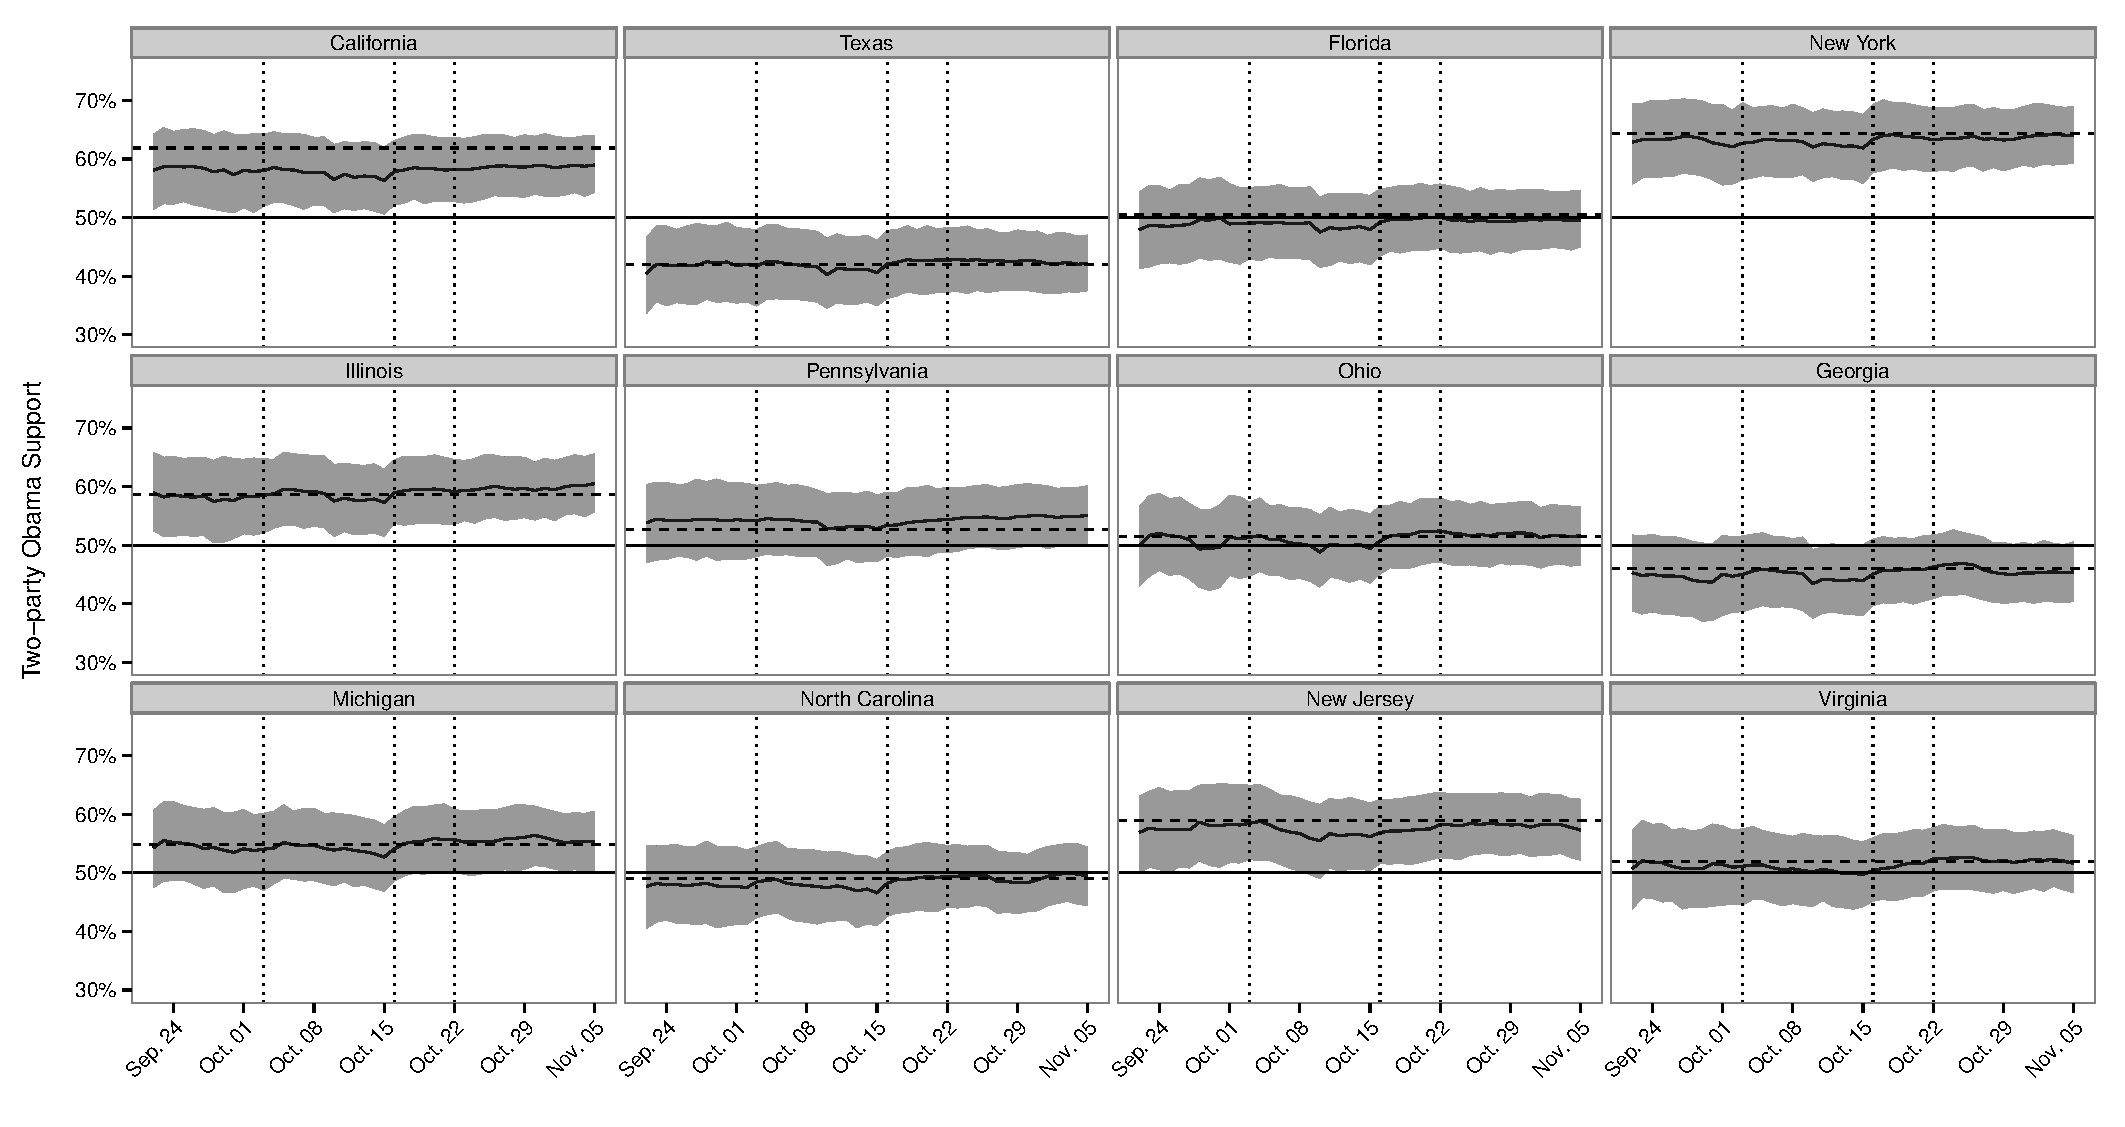
\includegraphics[width=\textwidth]{projected_voteshare_state}
  \caption{Projected Obama share of the two-party vote on election day
    for each of the 12 states
    with the most electoral votes, and associated 95\% confidence
    bands. Compared to the MRP-adjusted voter intent in Figure
    \ref{fig:state_snap}, the projected two-party Obama support is more stable, and the North Carolina race switches direction after applying the
    calibration model. Additionally, the confidence bands become much wider and
    give more reasonable state-by-state probabilities of Obama victories.}
  \label{fig:proj_state}
\end{figure}

\begin{figure}[p!]
  \centering
  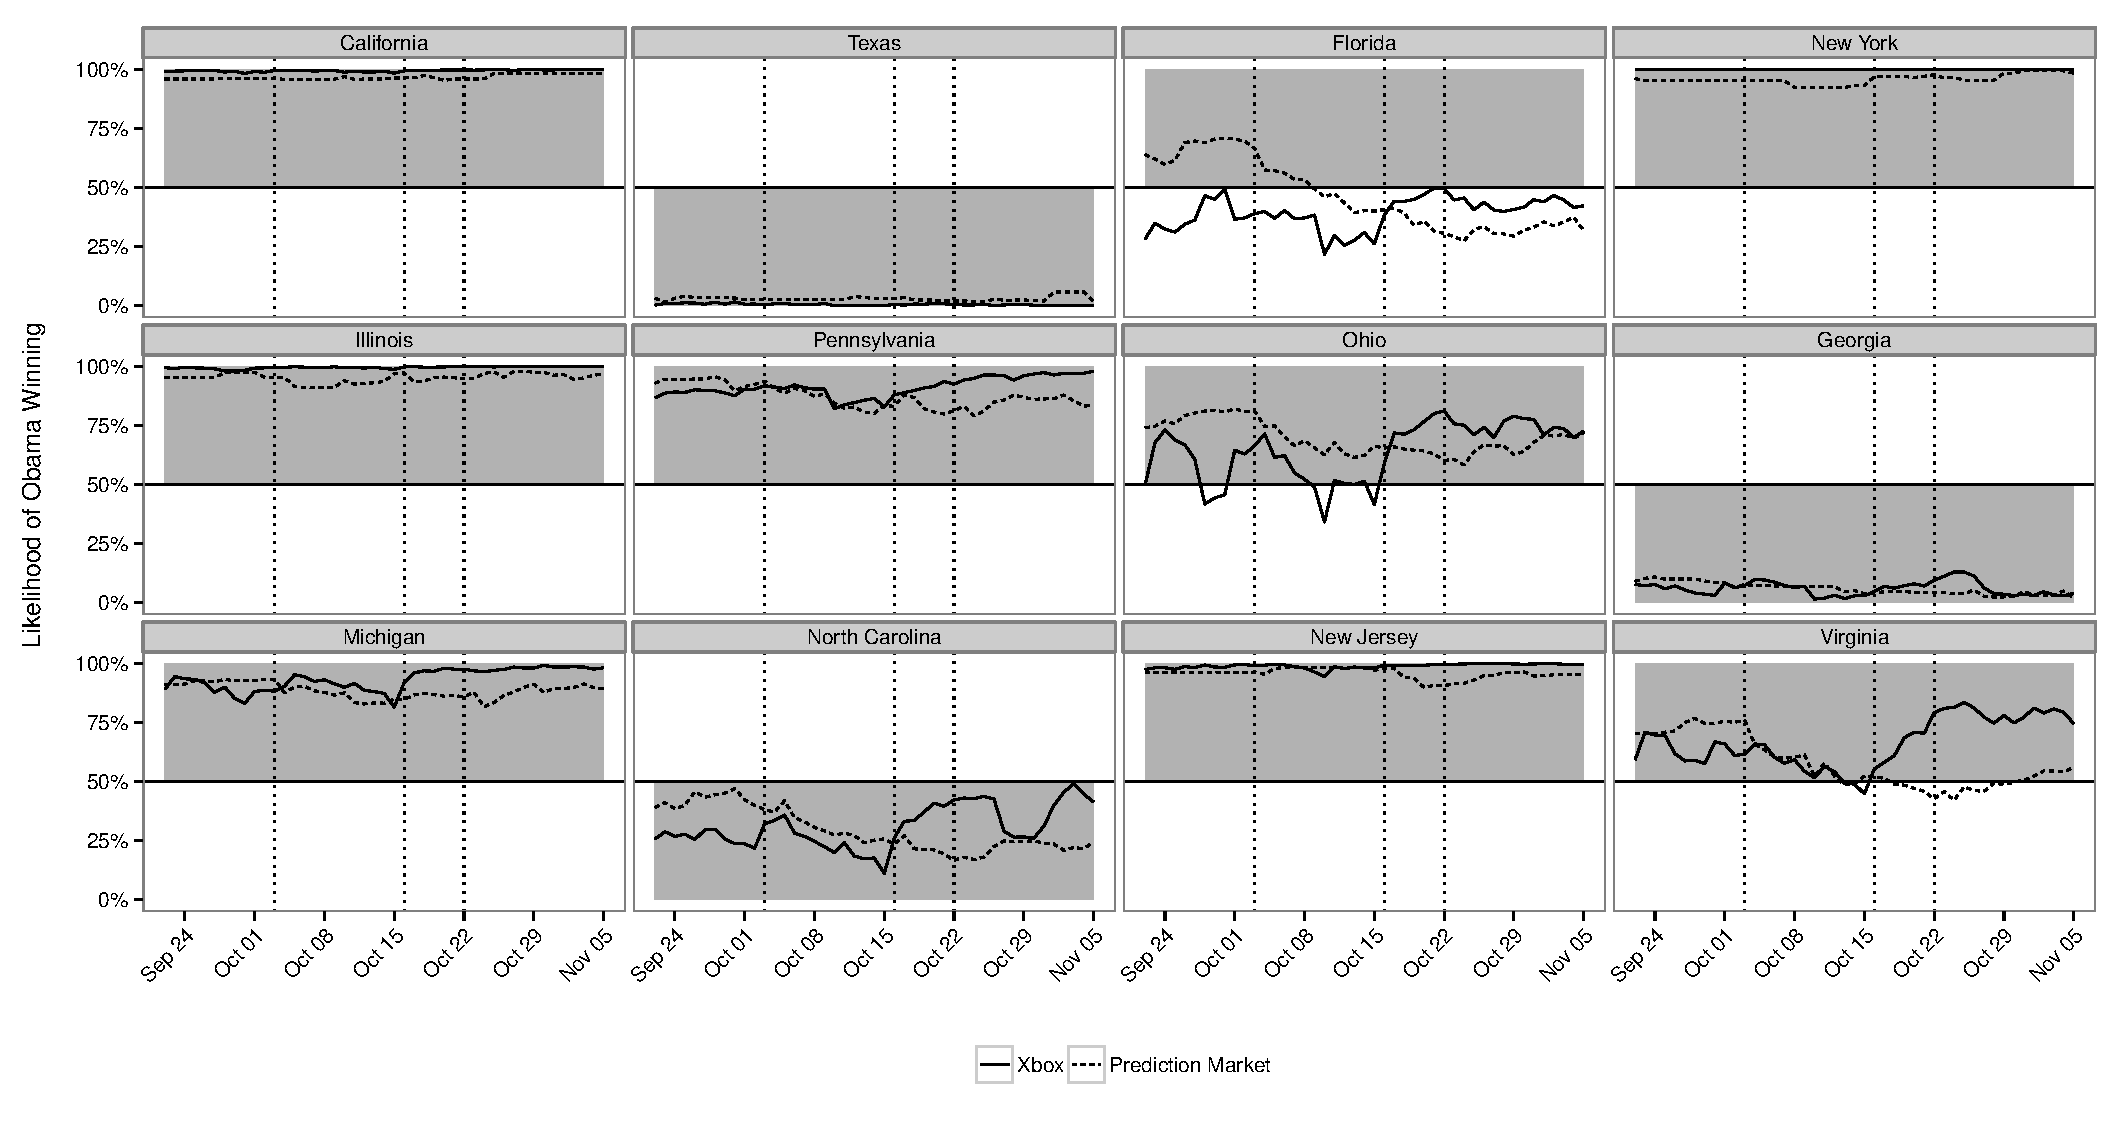
\includegraphics[width=\textwidth]{pred_market_xbox_comp}
  \caption{Comparison between the probability of Obama winning the 12 largest
    Electoral College races based on Xbox data and on prediction market
    data. The prediction market data are the average of the raw Betfair and Intrade
    prices from winner-take-all markets. The three vertical lines represent the
    dates of three presidential debates. The shaded halves indicate the direction
    that race went.}
  \label{fig:pm_comp}
\end{figure}

\begin{figure}[p!]
  \centering
  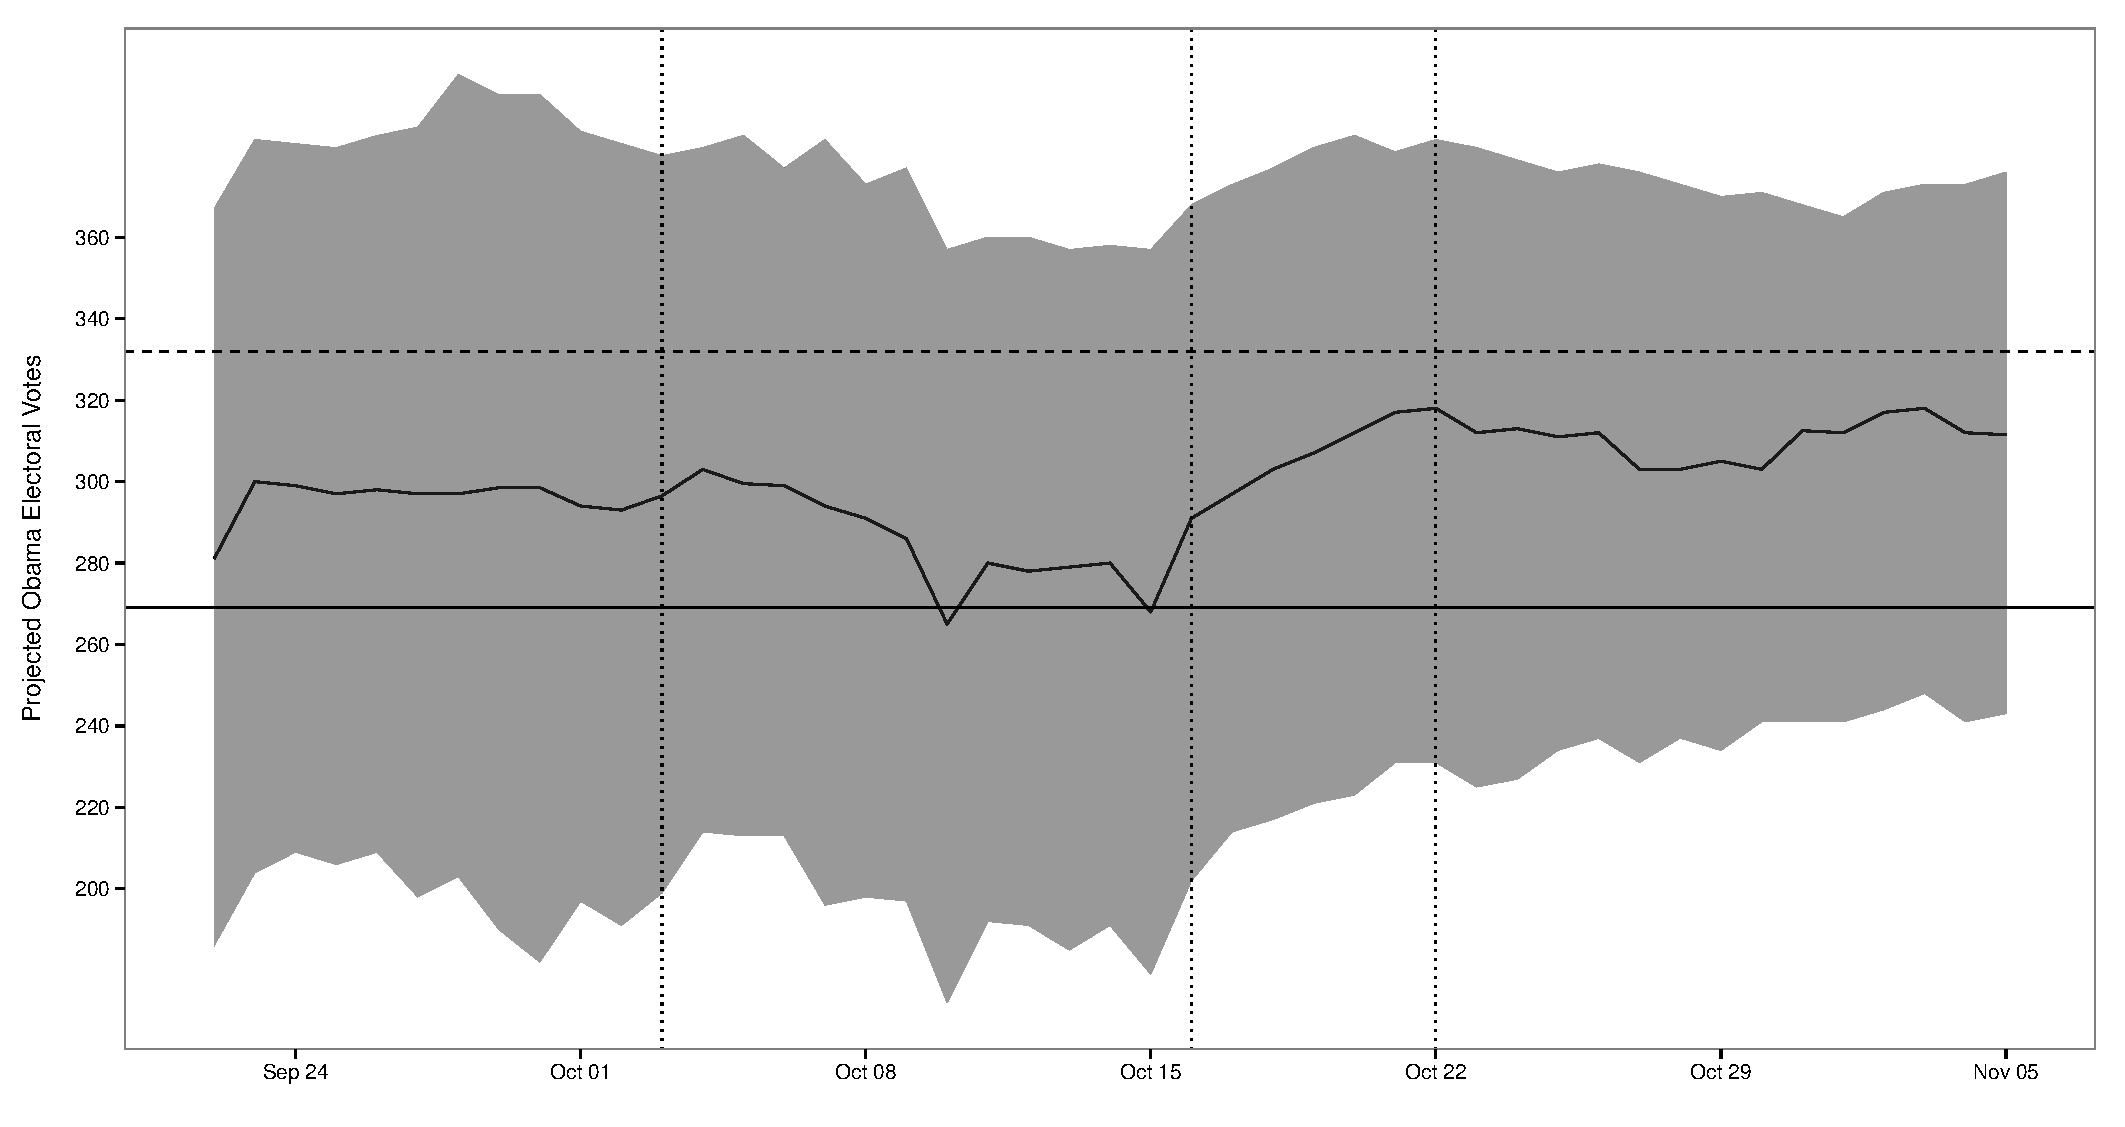
\includegraphics[width=\textwidth]{electoral_vote_dist_over_time}
  \caption{Daily projections of Obama electoral votes in the 45-day period
    leading up to the 2012 election and associated 95\% confidence bands. The
    solid line represents the median of the daily distribution. The horizontal
    dashed line represents the actual electoral votes, 332, that Obama captured
    in 2012 election. Three vertical dotted lines indicate the dates of three
    presidential debates.}
  \label{fig:ev_daily}
\end{figure}

\begin{figure}[p!]
  \centering
  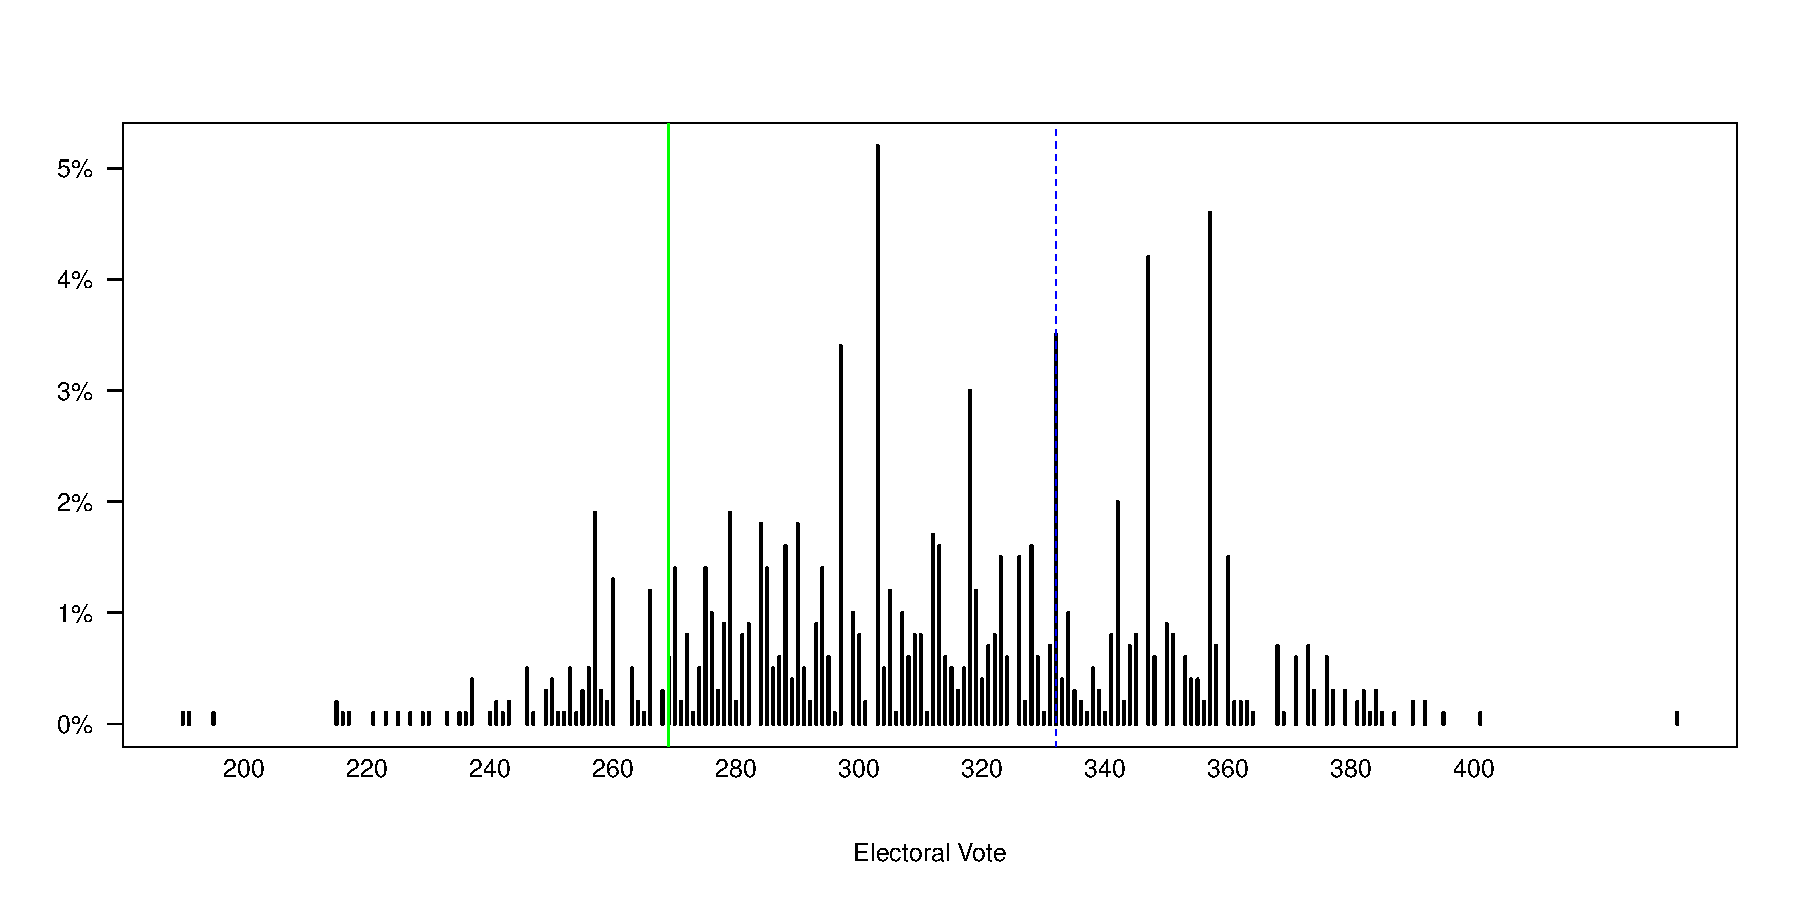
\includegraphics[width=\textwidth]{last_day_electoral_vote_dist}
  \caption{Projected distribution of electoral votes for Obama one day before the election. The green vertical dotted line represents 269, the minimum number of electoral votes that Obama needs for a tie. The blue vertical dashed line gives 332, the actual number of electoral votes captured by Obama. The estimated likelihood of Obama winning the electoral vote is 88\%.}
  \label{fig:ev_lastday}
\end{figure}

With the full state-level outcome distribution, I can also estimate the
distribution of Electoral College votes.
Figure\textasciitilde{}\ref{fig:ev_daily} plots the median projected
electoral votes for Obama over the last 45-days of the election,
together with the 95\% confidence band. In particular, on the day before
the election, my model estimates Obama had an 88\% chance of victory, in
line with estimates based on traditional polling data. For example,
Simon Jackman predicted Obama had a 91\% chance of victory, using a
method built from (Jackman 2005). Zooming in on the day before the
election, Figure\textasciitilde{}\ref{fig:ev_lastday} shows the full
predicted distribution of electoral votes for Obama. Compared to the
actual 332 votes that Obama captured, I estimate a median of 312 votes,
with the most likely outcome being 303. Though this distribution of
Electoral College outcomes seems reasonable, it does appear to have
higher variance than one might expect. In particular, the extreme
outcomes seem to have unrealistically high likelihood of occurring,
which is likely a byproduct of the calibration model not fully capturing
the state-level correlation structure. Nonetheless, given that my
forecasts are based on a highly biased convenience sample of
respondents, the model predictions are remarkably good.

\section{Conclusion}\label{conclusion}

Forecasts not only need to be accurate, but also relevant, timely, and
cost-effective. In this chapter, I construct election forecasts
satisfying all of these requirements using extremely non-representative
data. Though the data were collected on a proprietary polling platform,
in principle one can aggregate such non-representative samples at a
fraction of the cost of conventional survey designs. Moreover, the data
produce forecasts that are both relevant and timely, as they can be
updated faster and more regularly than standard election polls. Thus,
the key question---and one of the main contributions of this
chapter---is to assess the extent to which one can generate accurate
predictions from non-representative samples. Since there is limited
ground truth for election forecasts, definitely establishing the
accuracy of my predictions is difficult. Nevertheless, I show that the
MRP-adjusted and calibrated Xbox estimates are both intuitively
reasonably, and are also quite similar to those generated by more
traditional means.

The greatest impact of non-representative polling will likely not be for
presidential elections, but rather for smaller, local elections and
specialized survey settings, where it is impractical to deploy
traditional methods due to cost and time constraints. For example,
non-representative polls could be used in Congressional elections, where
there are currently only sparse polling data. Non-representative polls
could also supplement traditional surveys (e.g., the General Social
Survey) by offering preliminary results at shorter intervals. General
Social Survey, which is . Finally, when there is a need to identify and
track pivotal events that affect public opinion, non-representative
polling offers the possibility of cost-effective continuous data
collection. Standard representative polling will certainly continue to
be an invaluable tool for the foreseeable future. However, 75 years
after the \textsl{Literary Digest} failure, non-representative polling
(followed by appropriate post-data adjustment) is due for further
exploration, for election forecasting and in social research more
generally.

\hyperdef{}{references}{\label{references}}
\section*{Bibliography}\label{bibliography}
\addcontentsline{toc}{section}{Bibliography}

\hyperdef{}{ref-bates2013lme4}{\label{ref-bates2013lme4}}
Bates, Douglas, Martin Maechler, and Ben Bolker. 2013. \emph{Lme4:
Linear mixed-effects models using s4 classes}.
\url{http://CRAN.R-project.org/package=lme4}.

\hyperdef{}{ref-campbell2008american}{\label{ref-campbell2008american}}
Campbell, James E. 2008. 6 \emph{The american campaign: US presidential
campaigns and the national vote}. Texas A\&M University Press.

\hyperdef{}{ref-chen2008modeling}{\label{ref-chen2008modeling}}
Chen, M Keith, Jonathan E Ingersoll, and Edward H Kaplan. 2008.
``Modeling a presidential prediction market.'' \emph{Management Science}
54(8): 1381--1394.

\hyperdef{}{ref-erikson2008political}{\label{ref-erikson2008political}}
Erikson, Robert S, and Christopher Wlezien. 2008. ``Are political
markets really superior to polls as election predictors?'' \emph{Public
Opinion Quarterly} 72(2): 190--215.

\hyperdef{}{ref-gelman2007data}{\label{ref-gelman2007data}}
Gelman, Andrew, and Jennifer Hill. 2007. \emph{Data analysis using
regression and multilevel/hierarchical models}. Cambridge University
Press.

\hyperdef{}{ref-ghitzaux5f2013}{\label{ref-ghitzaux5f2013}}
Ghitza, Yair, and Andrew Gelman. 2013. ``Deep interactions with mRP:
Election turnout and voting patterns among small electoral subgroups.''
\emph{American Journal of Political Science} 57(3): 762--776.

\hyperdef{}{ref-gosnell1937technical}{\label{ref-gosnell1937technical}}
Gosnell, Harold F. 1937. ``How accurate were the polls?'' \emph{Public
Opinion Quarterly} 1(1): 97--105.

\hyperdef{}{ref-hillygus2009persuadable}{\label{ref-hillygus2009persuadable}}
Hillygus, D Sunshine, and Todd G Shields. 2009. \emph{The persuadable
voter: Wedge issues in presidential campaigns}. Princeton University
Press.

\hyperdef{}{ref-jackman2005pooling}{\label{ref-jackman2005pooling}}
Jackman, Simon. 2005. ``Pooling the polls over an election campaign.''
\emph{Australian Journal of Political Science} 40(4): 499--517.

\hyperdef{}{ref-kaufmann1999changing}{\label{ref-kaufmann1999changing}}
Kaufmann, Karen M, and John R Petrocik. 1999. ``The changing politics of
american men: Understanding the sources of the gender gap.''
\emph{American Journal of Political Science} 43(3): 864--887.

\hyperdef{}{ref-keeter2006gauging}{\label{ref-keeter2006gauging}}
Keeter, Scott et al. 2006. ``Gauging the impact of growing nonresponse
on estimates from a national rDD telephone survey.'' \emph{Public
Opinion Quarterly} 70(5): 759--779.

\hyperdef{}{ref-kohut2012assessing}{\label{ref-kohut2012assessing}}
Kohut, Andrew et al. 2012. ``Assessing the representativeness of public
opinion surveys.'' \emph{Pew Research Center for The People \& The
Press} 15(May): 2012.

\hyperdef{}{ref-laxux5f2009}{\label{ref-laxux5f2009}}
Lax, Jeffrey R, and Justin H Phillips. 2009. ``How should we estimate
public opinion in the states?'' \emph{American Journal of Political
Science} 53(1): 107--121.

\hyperdef{}{ref-little1993post}{\label{ref-little1993post}}
Little, Roderick JA. 1993. ``Post-stratification: A modeler's
perspective.'' \emph{Journal of the American Statistical Association}
88(423): 1001--1012.

\hyperdef{}{ref-lockux5f2010}{\label{ref-lockux5f2010}}
Lock, Kari, and Andrew Gelman. 2010. ``Bayesian combination of state
polls and election forecasts.'' \emph{Political Analysis} 18(3):
337--348.

\hyperdef{}{ref-park2004bayesian}{\label{ref-park2004bayesian}}
Park, David K, Andrew Gelman, and Joseph Bafumi. 2004. ``Bayesian
multilevel estimation with poststratification: State-level estimates
from national polls.'' \emph{Political Analysis} 12(4): 375--385.

\hyperdef{}{ref-nlme}{\label{ref-nlme}}
Pinheiro, Jose et al. 2012. \emph{Nlme: Linear and nonlinear mixed
effects models}.

\hyperdef{}{ref-rothschild2013combining}{\label{ref-rothschild2013combining}}
Rothschild, David. 2013. ``Combining forecasts: Accurate, relevant, and
timely.''

\hyperdef{}{ref-rothschild2009forecasting}{\label{ref-rothschild2009forecasting}}
Rothschild, David. 2009. ``Forecasting elections comparing prediction
markets, polls, and their biases.'' \emph{Public Opinion Quarterly}
73(5): 895--916.

\hyperdef{}{ref-squire19881936}{\label{ref-squire19881936}}
Squire, Peverill. 1988. ``Why the 1936 literary digest poll failed.''
\emph{Public Opinion Quarterly} 52(1): 125--133.

\hyperdef{}{ref-wang2014forecasting}{\label{ref-wang2014forecasting}}
Wang, Wei et al. 2014. ``Forecasting elections with non-representative
polls.'' \emph{International Journal of Forecasting}.

\hyperdef{}{ref-wolfers2004prediction}{\label{ref-wolfers2004prediction}}
Wolfers, Justin, and Eric Zitzewitz. 2004. \emph{Prediction markets}.
National Bureau of Economic Research.
